\section{Linear Discriminant Analysis}
Using Linear Discriminant Analysis we can overcome several problems with Logistic regression {  !!ref bog side 138!! }. When the classes are well-separated, the parameter estimates for the
logistic regression model are unstable. If our sample size is small and the distribution of the predictors X is a normal distribution in each of the classes, the linear discriminant model is again more better than the logistic regression model.
\subsection{Theory}
Before we start using LDA there is a  assumption about the data it operates on. Each of the predictors should be normal distributed for this to work properly. We see the formula used by LDA shown in \ref{fo:BayesTheorem}. Where $\pi_k$ is the prior probability that a randomly selected obsivation comes from the $k$th class. $f_k(x)$ is the probability density function of X for an observation that comes from the $k$th class. If the function is large then there is a high probability that an observation in the $k$th class.
\begin{align}\label{fo:BayesTheorem}
Pr(Y=k|X=x) = \frac{\pi_k f_k(x)}{ \sum_{l=1}^{k}\pi_l f_l(x) }
\end{align}
If we as a example choose to only use one predictor and we would like to obtain the estimate for $f_k(x)$ that we can use in \ref{fo:BayesTheorem} If we assume that $f_k(x)$ is a normal distribution and assume that variance is is same for all K classes \ref{fo:BayesTheoremWithNormal}.
\begin{align}\label{fo:BayesTheoremWithNormal}
Pk(x) = \frac{\pi_k \frac{1}{\sqrt{2\pi\sigma)}}\exp(-\frac{1}{2\sigma^2}(x-\mu_k)^2)}{ \sum_{l=1}^{k}\pi_l \frac{1}{\sqrt{2\pi\sigma)}}\exp(-\frac{1}{2\sigma^2}(x-\mu_l)^2) }
\end{align}
If we then take the log of \ref{fo:BayesTheoremWithNormal} and manipulate the terms we will arrive at \ref{fo:BayesTheoremAfterManipulateTheterms} this is the same as assigning the observation to the class for which is largest.
\begin{align}\label{fo:BayesTheoremAfterManipulateTheterms}
\delta_k = x\frac{\mu_k}{\sigma^2} - \frac{\mu^2_k}{2 \sigma^2} + \log(\pi_k)
\end{align}
In the example seen in Figure \ref{TwoOneDimensionalNormalDensityFunctions} The two probability density function that are displayed, f1(x) and f2(x), represent two distinct
classes. The mean and variance parameters for the two density functions. 
are $\mu=-1.25 \mu_2=1.25$ and $\sigma^2_1=\sigma^2_2=1$
\begin{figure}[h]
	\centering
	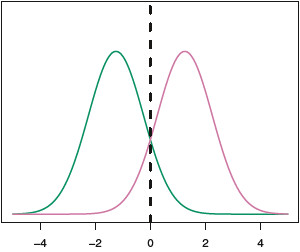
\includegraphics[scale=1.0]{discriminantAnalysis/linearDiscriminantAnalysis/fig/TwoOneDimensionalNormalDensityFunctions.jpg}
	\caption{Two normal distributions with the Bayes decision boundary in the middle.}
	\label{fig:TwoOneDimensionalNormalDensityFunctions}
\end{figure}



\subsection{Results}
In lab 4.6.3 We use Linear Discriminant Analysis. As we did in lab XXXX we split the data into before and after 2015 and then make training and testing data. Now that we have that out of the way it's time to import the Linear Discriminant Analysis from scikit-learn.
\begin{lstlisting}[language=Python]
from sklearn.discriminant_analysis import LinearDiscriminantAnalysis as LDA
\end{lstlisting}
Now the training process can begin.
\begin{lstlisting}[language=Python]
sklearn_lda = LDA(n_components=2) #creating a LDA object
lda = sklearn_lda.fit(X_train.iloc[:,1:3], y_train.iloc[:,1]) #learning the projection matrix
X_lda = lda.transform(X_train.iloc[:,1:3]) #using the model to project X. Project data to maximize class separation.
X_labels = lda.predict(X_train.iloc[:,1:3]) #gives you the predicted label for each sample
X_prob = lda.predict_proba(X_train.iloc[:,1:3]) #the probability of each sample to belong to each class
\end{lstlisting}
Now that the model have been fitted we will look at the coefficients of the model for Lag1 and Lag2.
\begin{lstlisting}[language=Python]
lda.coef_
array([[-0.05544078, -0.0443452 ]])
\end{lstlisting}
Now we will look at the priors. Therefor we can see that. $$ \hat{ \pi }_1 = -0.05544078  \hat{ \pi }_2 = -0.0443452 $$ 
\begin{lstlisting}[language=Python]
lda.priors_
array([ 0.49198397,  0.50801603])
\end{lstlisting}

Testing step. Now we will test out model using the data.
\begin{lstlisting}[language=Python]
X_test_labels=lda.predict(X_test.iloc[:,1:3])
X_test_prob = lda.predict_proba(X_test.iloc[:,1:3])
\end{lstlisting}

To Get the accuracy of the test set. We use the following command.

\begin{lstlisting}[language=Python]
np.mean(y_test.iloc[:,1]==X_test_labels)
0.55952380952380953
\end{lstlisting}

Let's change the threshod a bit to see whether we can improve the accuracy. The 2nd column of X\_test\_prob is the probability belongs to UP group. The default value is 0.5, let us first check that.

\begin{lstlisting}[language=Python]
threshold = 0.5 
np.mean(y_test.iloc[:,1]==(X_test_prob[:,1]>=threshold))
0.55952380952380953
\end{lstlisting}

